%% Royal Society Interface submission -- Supplementary Appendix (ESM)
%% Converted from paper/els-cas-paper/appendix.tex (2026-07-17); body content
%% is ported VERBATIM. Compiles STANDALONE (references to main-text
%% section/figure/table numbers are hard-coded, exactly as in the source).

%% Local-toolchain workaround (see main.tex): roll the kernel back so the
%% installed biblatex loads. Guarded so it stays a no-op on Overleaf/TeX Live,
%% where the unconditional form rolls graphics and amsmath back to 2019.
\IfFormatAtLeastTF{2026-01-01}{\RequirePackage[2025-06-01]{latexrelease}}{}

\documentclass[openacc]{rsproca_new}

%% Packages required by the appendix body (amsmath/amssymb/graphicx,
%% hyperref and biblatex are already loaded by the class).
\usepackage{booktabs}
\usepackage{multirow}
\usepackage{float}
\usepackage{placeins}
\usepackage{chngcntr}   % section-based float numbering (Figure A.1, Table B.1, ...)

%% Bibliography database (style is fixed by the class: biblatex/biber, phys)
\addbibresource{mybib.bib}

%% Numeric subsection numbering (A.1, B.1.1, ...) instead of the class default
%% "(a)"/"i": matches how the main text refers to appendix sections.
\renewcommand\thesubsection{\thesection.\arabic{subsection}}
\renewcommand\thesubsubsection{\thesubsection.\arabic{subsubsection}}

%% See main.tex: avoid \flushbottom stretching around large floats.
\raggedbottom

\jname{rsif}
\Journal{J R Soc Interface\ }

\begin{document}

\begin{center}
  {\LARGE\bfseries Supplementary Appendix}\\[6pt]
  {\large\itshape Payoff scaling shapes cooperation in LLM agents across languages}
\end{center}
\vspace{1.5em}

\appendix

% Number figures/tables as A.1, A.2, B.1, ... (reset per appendix section) so
% that references from the main paper (e.g. "Figure B.1") cannot be confused
% with the main text's own Figure/Table numbers.
\counterwithin{figure}{section}
\counterwithin{table}{section}

\section{Supplement to Methodology}\label{appendix:methodology}

\subsection{LLM configuration}\label{appendix:llm_config}

Table~\ref{tab:llm_config} summarises the configuration of LLM backends used in our experiments. Following the FAIRGAME protocol~\cite{buscemi2025fairgame}, we adopt each provider's recommended default settings to reflect realistic deployment conditions.

\begin{table}[!htbp]
\centering
\caption{LLM backend configurations. Temperature and sampling parameters follow each provider's recommended defaults. While this introduces potential variability confounds in cross-model comparisons, it reflects realistic deployment conditions where practitioners use models ``out of the box.''}
\label{tab:llm_config}
\footnotesize
\begin{tabular}{lccc}
\toprule
\textbf{Model} & \textbf{Provider} & \textbf{Temperature} & \textbf{Top\_p} \\
\midrule
GPT-4o            & OpenAI     & 1.0 & 1.0 \\
Claude 3.5 Haiku  & Anthropic  & 1.0 & 1.0 \\
Mistral Large     & Mistral AI & 0.3 & 1.0 \\
\bottomrule
\end{tabular}
\end{table}

\subsection{Payoff scaling examples}\label{appendix:payoff_scaling}

For illustration, the scaled payoff matrices under the three experimental conditions are shown below. When $\lambda = 0.1$ (attenuated stakes), the row player's payoff matrix becomes:
\[
\begin{array}{c|cc}
 & \text{Option A} & \text{Option B} \\
\hline
\text{Option A} & (0.6, 0.6) & (0, 1.0) \\
\text{Option B} & (1.0, 0)   & (0.2, 0.2)
\end{array}
\]
When $\lambda = 10.0$ (amplified stakes), it becomes:
\[
\begin{array}{c|cc}
 & \text{Option A} & \text{Option B} \\
\hline
\text{Option A} & (60, 60) & (0, 100) \\
\text{Option B} & (100, 0) & (20, 20)
\end{array}
\]
The ordering $T < R < P < S$ is preserved in all cases, ensuring the strategic structure of the Prisoner's Dilemma remains unchanged while only the magnitude of incentives varies.

\subsection{Rule-based strategy assignment}\label{appendix:rule_based}

To complement the LSTM-based strategy predictions and address cases where behavioural patterns exhibit characteristics of multiple canonical strategies, we apply deterministic rule-based algorithms to identify all potential strategy labels consistent with observed action sequences. These rules encode the defining characteristics of each strategy as logical conditions on the agent's action trajectory $\mathbf{a} = (a_1, a_2, \ldots, a_T)$ and the opponent's history $\mathbf{o} = (o_1, o_2, \ldots, o_T)$.

\textbf{Always Cooperate (ALLC).} The agent cooperates in all rounds regardless of opponent behaviour:
\[
\text{ALLC} \equiv \forall t \in \{1, \ldots, N\}: a_t = C
\]

\textbf{Always Defect (ALLD).} The agent defects in all rounds regardless of opponent behaviour:
\[
\text{ALLD} \equiv \forall t \in \{1, \ldots, N\}: a_t = D
\]

\textbf{Tit-for-Tat (TFT).} The agent cooperates in round 1, then copies the opponent's previous action. To accommodate execution errors, we tolerate up to $\epsilon_{\text{noise}}$ deviations from pure TFT logic:
\[
\text{TFT} \equiv (a_1 = C) \land \left(\sum_{t=2}^{N} \mathbb{I}[a_t \neq o_{t-1}] \leq \epsilon_{\text{noise}} \cdot (N-1)\right)
\]
where $\mathbb{I}[\cdot]$ is the indicator function and $\epsilon_{\text{noise}} = 0.1$ in our implementation.

\textbf{Win-Stay-Lose-Shift (WSLS).} The agent repeats its previous action if the outcome was a Reward ($R$, mutual cooperation) or Temptation ($T$, successful defection), and switches otherwise. The initial action can be either $C$ or $D$. Similarly, we tolerate up to $\epsilon_{\text{noise}}$ deviations:
\begin{equation*}
\begin{split}
& \text{Let } \hat{a}_t =
    \begin{cases}
        a_{t-1} & \text{if } (a_{t-1}, o_{t-1}) \in \{(C,C), (D,C)\} \\
        \neg a_{t-1} & \text{if } (a_{t-1}, o_{t-1}) \in \{(C,D), (D,D)\}
    \end{cases} \\
& \text{WSLS} \equiv \sum_{t=2}^{N} \mathbb{I}\left[a_t \neq \hat{a}_t\right] \leq \epsilon_{\text{noise}} \cdot (N-1)
\end{split}
\end{equation*}

These rules are applied sequentially to each trajectory. A trajectory may receive multiple labels if it satisfies conditions for overlapping strategies (e.g., a short sequence of all-cooperate satisfies both ALLC and TFT, and a short sequence of all-defect satisfies both ALLD and TFT). The hybrid pipeline combines these rule-based assignments with LSTM predictions: high-confidence LSTM outputs ($\tau \ge 0.9$) are retained, while ambiguous cases ($\tau < 0.9$) are supplemented with rule-based labels when applicable. Whenever the rule set fires on more than one canonical strategy, we retain all matched labels as a \emph{composite} label of the form ``ALLD$|$TFT'' or ``ALLC$|$TFT$|$WSLS'' rather than collapsing to a single ``priority'' strategy; in our corpus, approximately $24.4\%$ of high-confidence proprietary trajectories receive such a composite label (see Appendix~\ref{appendix:mixture_labels} for the per-pattern breakdown). For aggregate statistics, every composite label is then expanded into one row per matched strategy before normalising, so a trajectory whose rule set fires on ALLC, TFT and WSLS contributes equal mass to each of the three. This approach ensures both coverage (via rules for unambiguous patterns) and robustness (via LSTM for noisy, complex cases).

\subsection{High-confidence filtering rationale}\label{appendix:filtering_rationale}

We employed a selective filtering approach to ensure the reliability of our LLM behavioural strategy analysis. Specifically, we focused our analysis on game instances where the predicted strategy labels for both agents exhibited prediction probabilities exceeding $0.9$ (90\% confidence threshold). The decision to use high-confidence predictions is grounded in several key considerations:
\begin{itemize}
    \item \textbf{Pattern alignment with theoretical strategies:} Samples with prediction probabilities above $0.9$ indicate that the observed behavioural sequences of LLMs closely align with the canonical patterns defined by the four classical strategies (ALLD, ALLC, WSLS, and TFT).
    \item \textbf{Signal-to-noise separation:} While the probabilities are not absolute (not reaching $1.0$), this is expected and attributable to inherent noise in LLM decision-making processes.
    \item \textbf{Statistical reliability:} By focusing on high-confidence predictions, we minimise the risk of misclassification and ensure that our strategy distribution analysis reflects genuine behavioural patterns.
\end{itemize}

\subsection{Threshold sensitivity analysis}\label{appendix:threshold_sensitivity}

To validate our choice of confidence threshold $\tau = 0.9$, we conducted a systematic sensitivity analysis across $\tau \in [0.3, 0.95]$ for 3-, 4-, and 5-strategy classification models. Figure~\ref{fig:threshold_sensitivity} illustrates how retention rate, average confidence, number of predictions retained, and strategy diversity vary as a function of threshold value.

\begin{figure}[!htbp]
    \centering
    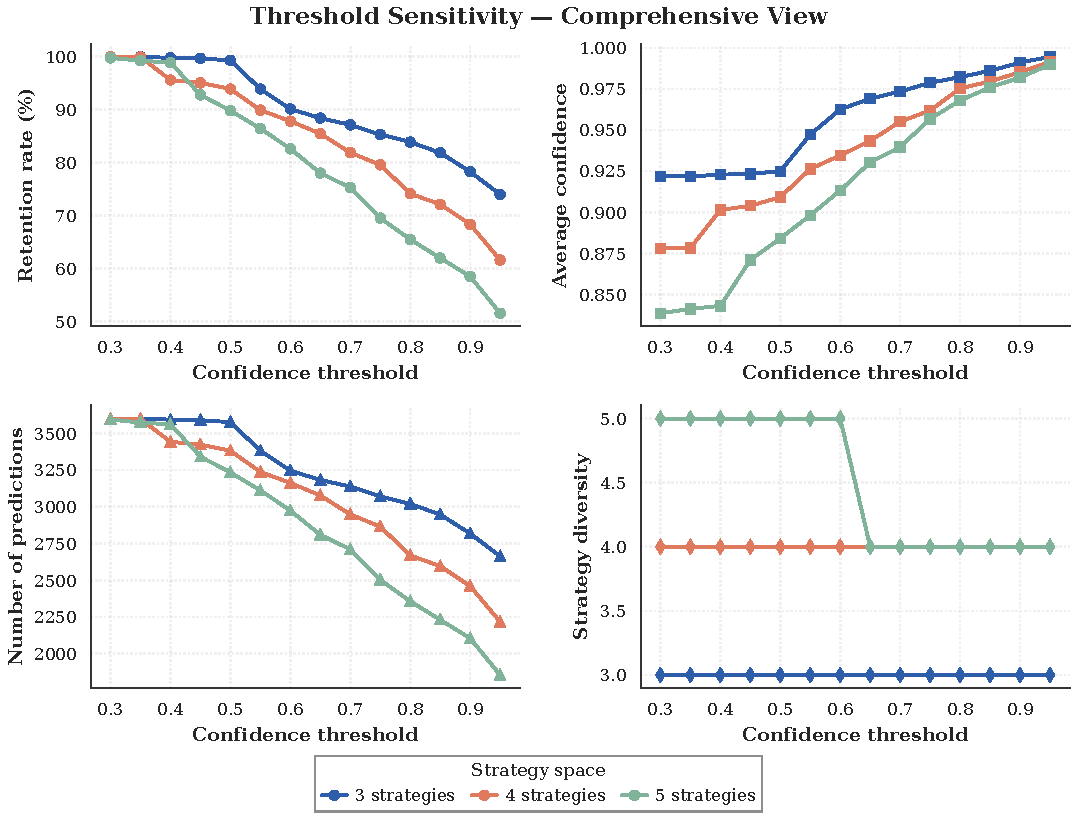
\includegraphics[width=\linewidth]{all_figures/fig05_threshold_combined_metrics.pdf}
    \caption{Comprehensive threshold sensitivity analysis for payoff-scaled experiments. Top row: retention rate and average confidence vs.\ threshold. Bottom row: number of predictions retained and strategy diversity. The 4-strategy model at $\tau = 0.9$ provides optimal balance between coverage and reliability (avg.\ confidence $0.985$). Note that $68.3\%$ is the LSTM-only retention at this threshold; the full hybrid pipeline (Section~2.3) reaches ${\approx}81\%$ by supplementing low-confidence LSTM cases with rule-based labels.}
    \label{fig:threshold_sensitivity}
\end{figure}

Table~\ref{tab:threshold_comparison} summarises key metrics at $\tau = 0.9$.

\begin{table}[!htbp]
\centering
\caption{Threshold sensitivity at $\tau = 0.9$ across strategy models.}
\label{tab:threshold_comparison}
\footnotesize
\begin{tabular}{lccc}
\toprule
\textbf{Metric} & \textbf{3-Strat} & \textbf{4-Strat} & \textbf{5-Strat} \\
\midrule
Retention Rate & 78.3\% & 68.3\% & 58.5\% \\
Avg. Confidence & 0.991 & 0.985 & 0.982 \\
Diversity & 3 & 4 & 4 \\
\bottomrule
\end{tabular}
\end{table}

Key findings: (1) Retention rate decreases as strategy space expands, reflecting greater behavioural complexity; (2) Average confidence remains $>0.97$ at $\tau = 0.9$ across all models; (3) Lowering to $\tau = 0.7$ would increase retention to $75$--$87\%$ but reduce average confidence to $0.94$--$0.97$. Our choice of $\tau = 0.9$ prioritises classification reliability while maintaining sufficient coverage for statistical analysis.

Table~\ref{tab:tau_sweep_distribution} reports the inferred strategy distribution on the proprietary corpus across $\tau \in \{0.7, 0.8, 0.9, 0.95\}$, computed under the same composite-label expansion as Table~1 so the two tables are directly comparable. The qualitative picture is essentially invariant: retention drops from $90.8\%$ to $75.5\%$ as the threshold rises, but the per-strategy frequencies move by less than one percentage point anywhere in the table, and the rank ordering of the four strategies is preserved at every threshold. This is direct evidence that the substantive conclusions of Section~3.2 are not artefacts of the specific confidence cutoff chosen.

\begin{table}[!htbp]
\centering
\caption{Threshold sweep for the proprietary corpus: retention rate and inferred strategy frequencies across $\tau \in \{0.7, 0.8, 0.9, 0.95\}$, computed with composite-label expansion (Appendix~\ref{appendix:mixture_labels}). The $\tau \geq 0.9$ row matches the overall row of Table~1. The distribution is essentially stationary in $\tau$, and the rank ordering of the four strategies is preserved.}
\label{tab:tau_sweep_distribution}
\footnotesize
\begin{tabular}{lccccc}
\toprule
$\tau$ & Retention (\%) & ALLC (\%) & ALLD (\%) & TFT (\%) & WSLS (\%) \\
\midrule
0.70 & 90.83 & 28.25 & 25.93 & 21.53 & 24.28 \\
0.80 & 86.22 & 28.67 & 26.18 & 21.23 & 23.92 \\
0.90 & 80.94 & 29.05 & 25.86 & 21.06 & 24.03 \\
0.95 & 75.50 & 28.83 & 25.22 & 21.48 & 24.48 \\
\bottomrule
\end{tabular}
\end{table}

\subsection{Classifier robustness across noise and strategy space}\label{appendix:robustness_noise}

This appendix benchmarks the LSTM intent recogniser used throughout the paper. Two complementary views are reported: (i) how the LSTM scales as the strategy space grows from 3 to 5 canonical strategies (Figure~\ref{fig:model_performance}), and (ii) how the LSTM compares against Logistic Regression and Random Forest baselines under execution noise (Figure~\ref{fig:model_robustness_appendix}).

\begin{figure}[!htbp]
    \centering
    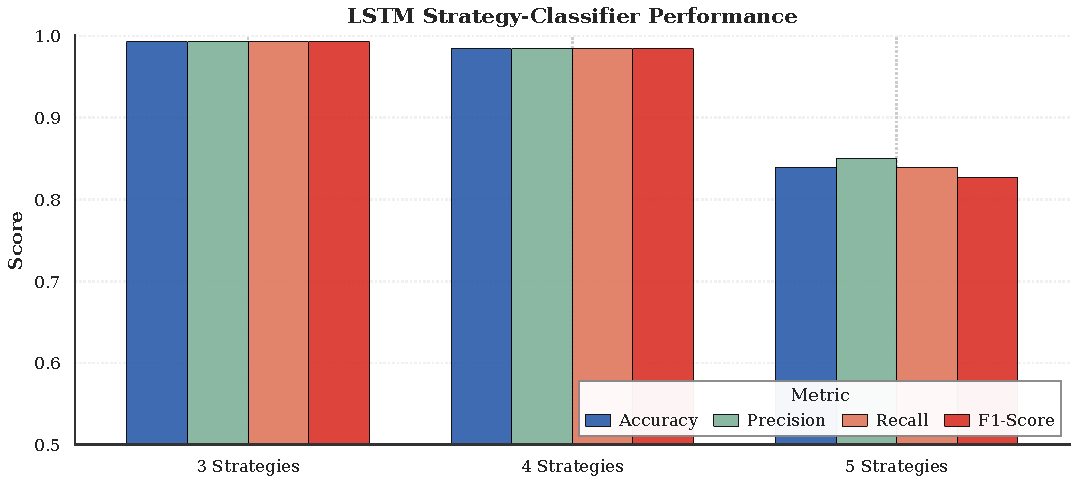
\includegraphics[width=\linewidth]{all_figures/fig01_lstm_model_performance.pdf}
    \caption{\textbf{LSTM intent recogniser performance across strategy-space sizes.} Accuracy, precision, recall and F1-score on synthetic trajectories with $5\%$ execution noise. F1 ranges from $0.984$ (4-strategy task) to $0.83$ (5-strategy task); all main-text analyses use the 4-strategy classifier ($\text{F1} = 0.984$).}
    \label{fig:model_performance}
\end{figure}

Figure~\ref{fig:model_performance} confirms the LSTM maintains robust performance even as the strategy space expands, successfully distinguishing between behaviourally similar conditional strategies (Tit-for-Tat and Win-Stay--Lose-Shift) within our analysed set of four canonical strategies. The recurrent architecture's ability to filter execution noise common in LLM outputs makes it particularly well-suited for this task~\cite{diStefanoIntention2023,Han2012ALIFEjournal}.

\begin{figure}[!htbp]
    \centering
    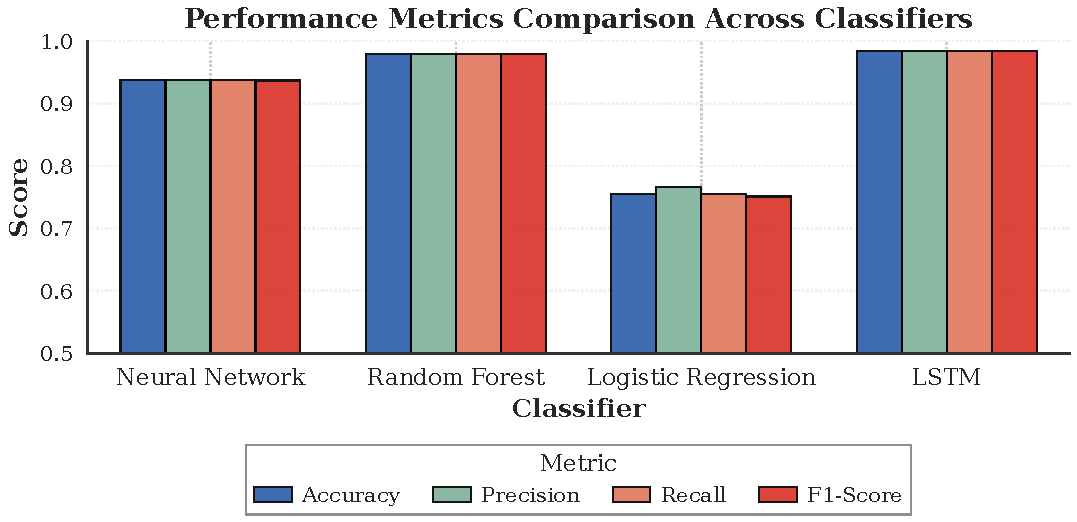
\includegraphics[width=\linewidth]{all_figures/fig06_classifier_performance_comparison.pdf}
    \caption{Model robustness to noise. Comparison of accuracy and F1-score between Logistic Regression, Random Forest, and LSTM on no-noise and noise $0.05$ datasets. The LSTM demonstrates superior resilience to execution noise.}
    \label{fig:model_robustness_appendix}
\end{figure}

We also evaluated the robustness of different classifier architectures against execution noise, which simulates the stochasticity and potential ``hallucinations'' of LLMs. As shown in Figure~\ref{fig:model_robustness_appendix}, while Logistic Regression (LR) and Random Forest (RF) models achieved near-perfect accuracy (greater than $0.9$) on clean data, their performance degraded when introduced to $5\%$ execution noise. In contrast, the Long Short-Term Memory (LSTM) network maintained the highest accuracy ($\sim 94\%$). This superiority stems from the LSTM's recurrent architecture, which allows it to learn the sequential ``context'' of a strategy, effectively ``forgiving'' random deviations to identify the core behavioural pattern.

\section{Supplement to Results}\label{appendix:results}

\subsection{Payoff-scaled experiments: additional analyses}\label{appendix:payoff_scaled}

This section provides supplementary analyses for the payoff-scaled Prisoner's Dilemma experiments (see main paper).

\subsubsection{Per-stake behavioural metrics}\label{appendix:per_multiplier_metrics}

To visualise the behavioural profiles of different LLM architectures across payoff scaling conditions, we present radar charts comparing normalised metrics for each stake/multiplier setting. Figure~\ref{fig:per_multiplier_radar} displays four key behavioural dimensions - internal variability (IV), cross-language inconsistency (CI), variability over round (VR), and sensitivity-to-payoff (SP) - normalised within each multiplier condition to enable direct cross-model comparison.

\begin{figure}[!htbp]
    \centering
    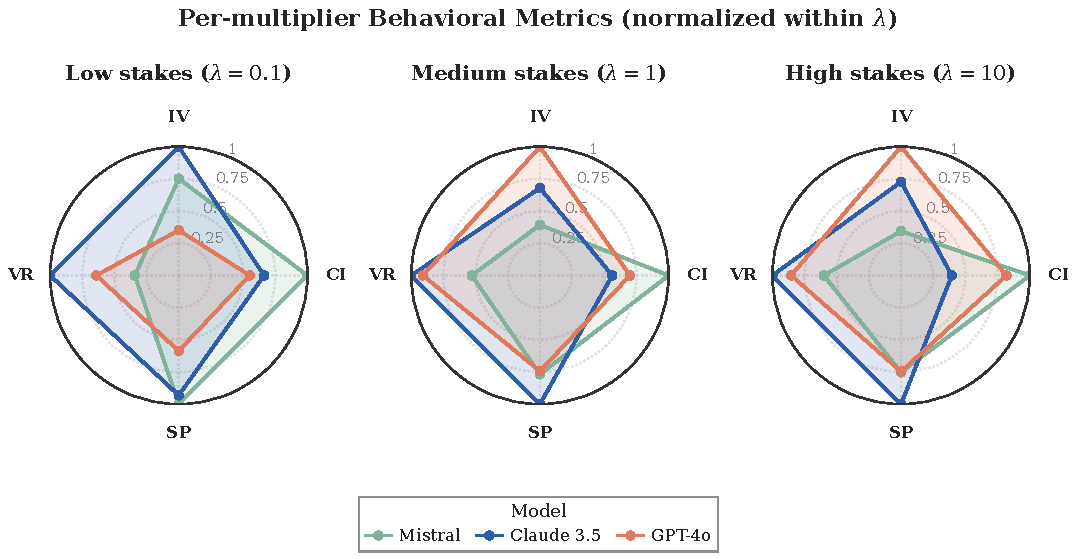
\includegraphics[width=\linewidth]{all_figures/fig07_per_lambda_radar.pdf}
    \caption{\textbf{Per-multiplier behavioural metrics.} We report four standardised metrics defined in the FAIRGAME framework~\cite{buscemi2025fairgame}: (1) \textbf{Internal Variability (IV)}, which quantifies the stochasticity of an agent's behaviour by measuring the variance of outcomes across identical experimental repetitions; (2) \textbf{Cross-Language Inconsistency (CI)}, which measures the standard deviation of agent performance across the five tested languages to indicate sensitivity to linguistic framing; (3) \textbf{Variability over Round (VR)}, which captures the volatility of decision-making and strategy changes throughout the 10-round game horizon; and (4) \textbf{Sensitivity-to-Payoff (SP)}, which reflects the magnitude of behavioural adaptation in response to varying incentive stakes. Radar charts compare Mistral Large (green), Claude 3.5 Haiku (orange), and GPT-4o (blue) across three payoff scales ($\lambda \in \{0.1, 1, 10\}$). Compared to the baseline payoff ($\lambda=1$), similar scores are observed for the higher stake payoff ($\lambda=10$). At low stakes ($\lambda=0.1$), models exhibit divergent scores. Overall, internal variability (IV) is most affected by varying the payoff stake.}
    \label{fig:per_multiplier_radar}
\end{figure}

Key observations include: (1) at attenuated stakes ($\lambda=0.1$), the three models display maximally divergent behavioural signatures, with Claude~3.5~Haiku exhibiting elevated variation rate while GPT-4o shows stronger cooperation index; (2) at baseline stakes ($\lambda=1$), models begin to converge toward more balanced profiles; (3) at amplified stakes ($\lambda=10$), all models shift toward higher CI and SP values, suggesting that increased consequences promote both cooperative behaviour and strategic consistency. These radar visualisations complement the line plots in the main paper by providing a holistic view of multi-dimensional behavioural shifts.

\begin{figure}[!htbp]
    \centering
    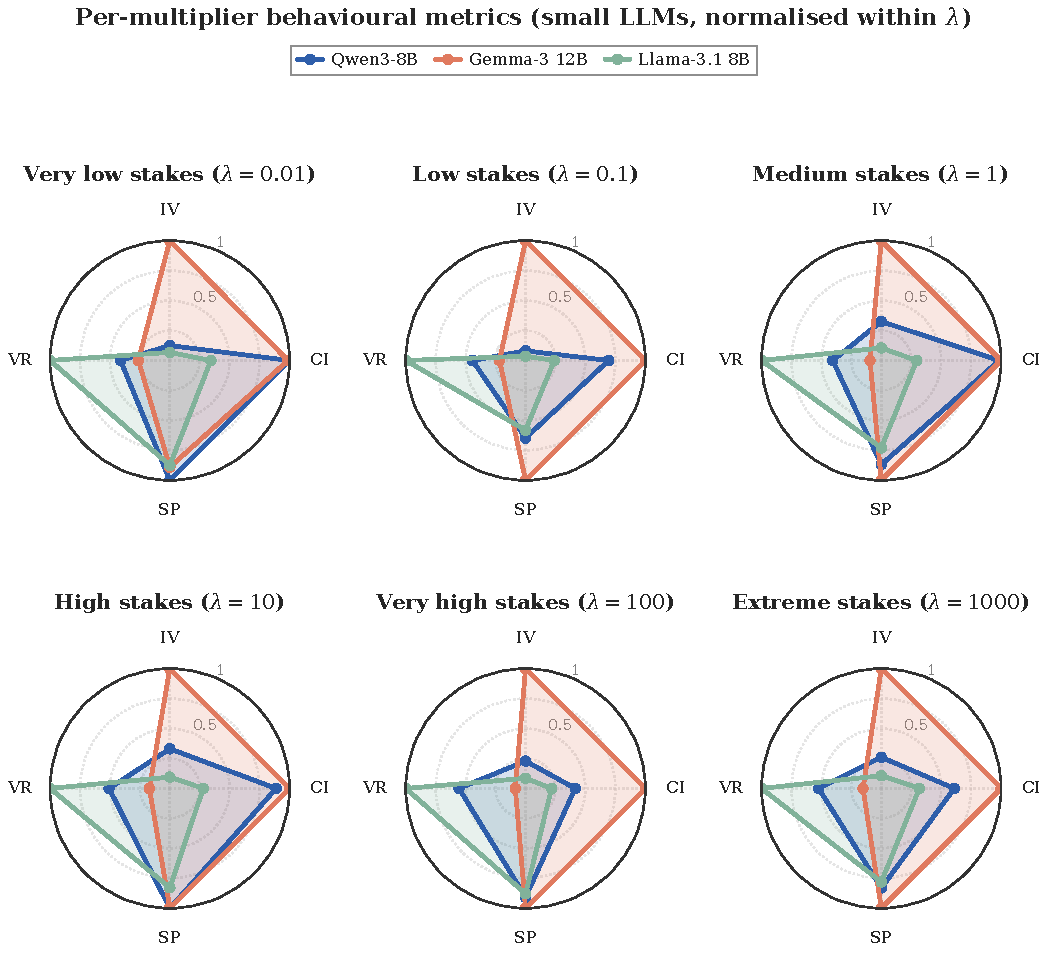
\includegraphics[width=\linewidth]{all_figures/ijcai_radar_chart_6multipliers_small_llm.pdf}
    \caption{\textbf{Per-multiplier behavioural metrics for the open-weight small LLMs.} The four standardised FAIRGAME metrics (IV, CI, SP, VR) -- defined identically to Figure~\ref{fig:per_multiplier_radar} and computed directly from the round-by-round OptionA/OptionB decisions in \texttt{Dataset/data\_fairgame\_small\_llm/} -- are reported for Qwen3~8B (blue), Gemma-3~12B (orange), and Llama-3.1~8B (green) across all six payoff scales covered by the small-LLM corpus ($\lambda \in \{0.01, 0.1, 1, 10, 100, 1000\}$). Each panel is normalised within $\lambda$ (divide-by-max across the three models), matching the proprietary radar so that the two figures can be read side by side. Two regime patterns are visible across the full sweep: Gemma-3~12B exhibits the largest internal variability (IV) at every $\lambda$, indicating the most stochasticity across identical repetitions, while Llama-3.1~8B exhibits the largest within-trace volatility (VR), indicating frequent round-by-round switching. Cross-language inconsistency (CI) peaks at very high stakes ($\lambda \geq 100$) and, like the proprietary panel, the sensitivity-to-payoff proxy (SP) compresses toward the upper end as stakes grow.}
    \label{fig:small_radar}
\end{figure}

\subsubsection{Multidimensional behavioural comparison}\label{appendix:multidimensional}

The visualisation in Figure~\ref{fig:multidimensional_behaviour} provides a synoptic view of how the three cardinal dimensions of our study - payoff magnitude, linguistic context, and model architecture - interact to shape agent behaviour. By synthesising these factors, we observe that strategic behaviour is not driven by a single determinant but emerges from their complex interplay. Notably, the variance attributable to linguistic context (visualised across the language axes) often rivals or even exceeds the variance between distinct model architectures, challenging the notion of fixed, immutable ``model personalities.'' Furthermore, the impact of payoff scaling is shown to be non-uniform; while amplified stakes generally compress behavioural diversity towards cooperation, the specific trajectory of this shift is heavily modulated by the language in which the game is framed. This suggests that alignment interventions must account for this multidimensional sensitivity, as a model aligned for safety in English may exhibit divergent, risk-seeking behaviours when prompted in other languages or under different incentive structures.

\begin{figure}[!htbp]
    \centering
    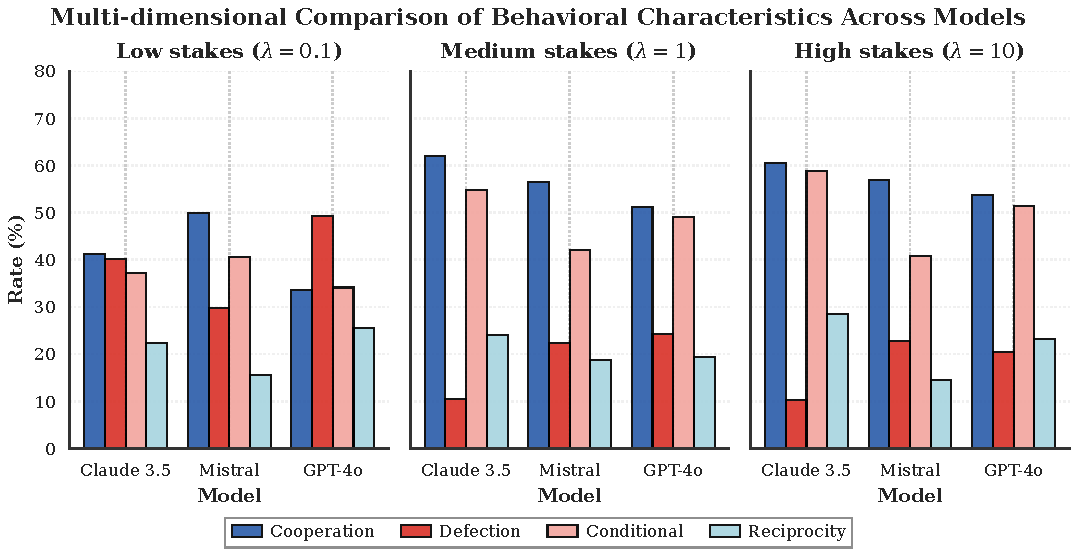
\includegraphics[width=\linewidth]{all_figures/fig16_behavioral_characteristics.pdf}
    \caption{Multidimensional comparison of LLM behavioural strategies across payoff scales, languages, and model architectures. The figure synthesises incentive sensitivity, linguistic priming, and architectural bias, illustrating that language effects can rival or exceed model-level differences.}
    \label{fig:multidimensional_behaviour}
\end{figure}

\begin{figure}[!htbp]
    \centering
    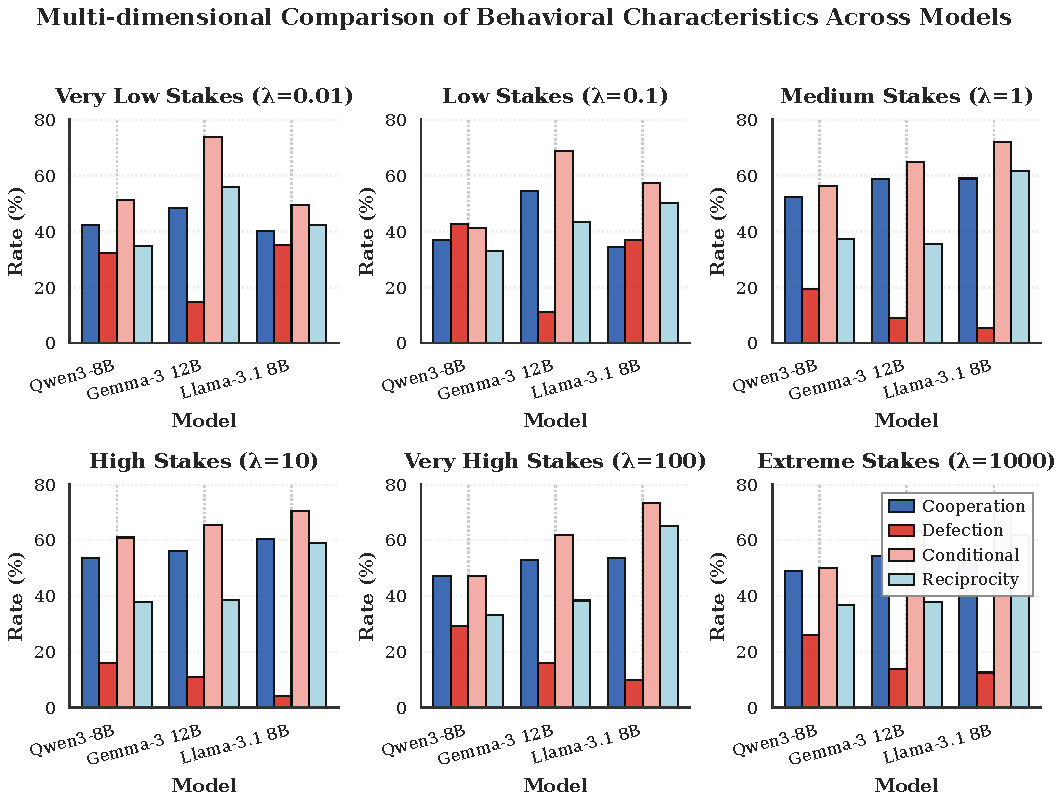
\includegraphics[width=\linewidth]{all_figures/ijcai_multidimensional_behavioral_comparison_small_llm.pdf}
    \caption{\textbf{Multidimensional behavioural comparison of the open-weight small LLMs across payoff scales, languages, and model architectures.} The figure synthesises incentive sensitivity, linguistic priming, and architectural bias in the same way as Figure~\ref{fig:multidimensional_behaviour} for the proprietary models. Language effects again rival or exceed model-level differences, and the impact of payoff scaling is heavily modulated by the prompt language.}
    \label{fig:small_multidim}
\end{figure}

\subsubsection{Unconditional vs.\ conditional strategy aggregation}\label{appendix:uncond_cond}

To provide a higher-level view of strategic tendencies across linguistic contexts, we aggregate the four canonical strategies into two categories: \emph{unconditional} (ALLC + ALLD) and \emph{conditional} (TFT + WSLS). This aggregation reveals whether agents commit to fixed policies regardless of opponent behaviour, or adapt their strategies based on interaction history.

\begin{figure}[!htbp]
    \centering
    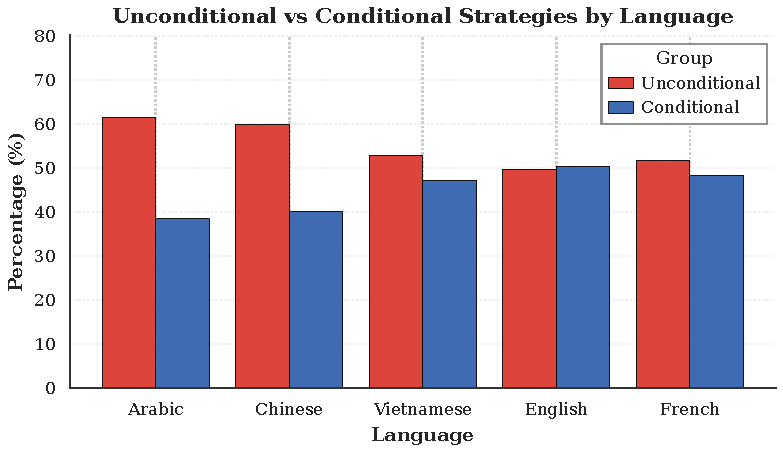
\includegraphics[width=0.7\linewidth]{all_figures/fig09_uncond_vs_cond_by_lang.pdf}
    \caption{Unconditional versus conditional strategy aggregation across languages (payoff-scaled experiments). Arabic and Chinese exhibit the highest unconditional rates, while English, French, and Vietnamese sit near a balanced split. This aggregated view complements the language strategy distribution table in the main paper.}
    \label{fig:language_strategy_grouped}
\end{figure}

As shown in Figure~\ref{fig:language_strategy_grouped}, Arabic and Chinese prompts elicit predominantly unconditional behaviour, while English, French, and Vietnamese sit close to a balanced split between unconditional and conditional play. This pattern corroborates the fine-grained analysis in the main paper, suggesting that linguistic context systematically modulates the degree to which LLM agents engage in adaptive versus committed strategic behaviour.

\subsubsection{Per-condition penalty breakdown (proprietary models)}\label{appendix:proprietary_per_condition}

The compact cooperation-rate view in the main text (Figure~2) is summarised from a much richer underlying dataset that crosses three stake regimes, five languages, three personality pairings and three proprietary models. Figure~\ref{fig:total_penalties_appendix} reports the per-cell mean penalties at the three stake regimes shown in the main text. Two design choices are visible immediately: agents incur lower penalties at higher stakes when measured in normalised units (because the cooperative outcome is rewarded relatively more), and personality framing shifts behaviour systematically (cooperative--cooperative pairings consistently incur lower penalties than selfish--selfish ones). The Arabic prompts elicit elevated defection in cooperative pairings -- the ``Arabic anomaly'' that also appears in the open-weight corpus.

\begin{figure}[!htbp]
    \centering
    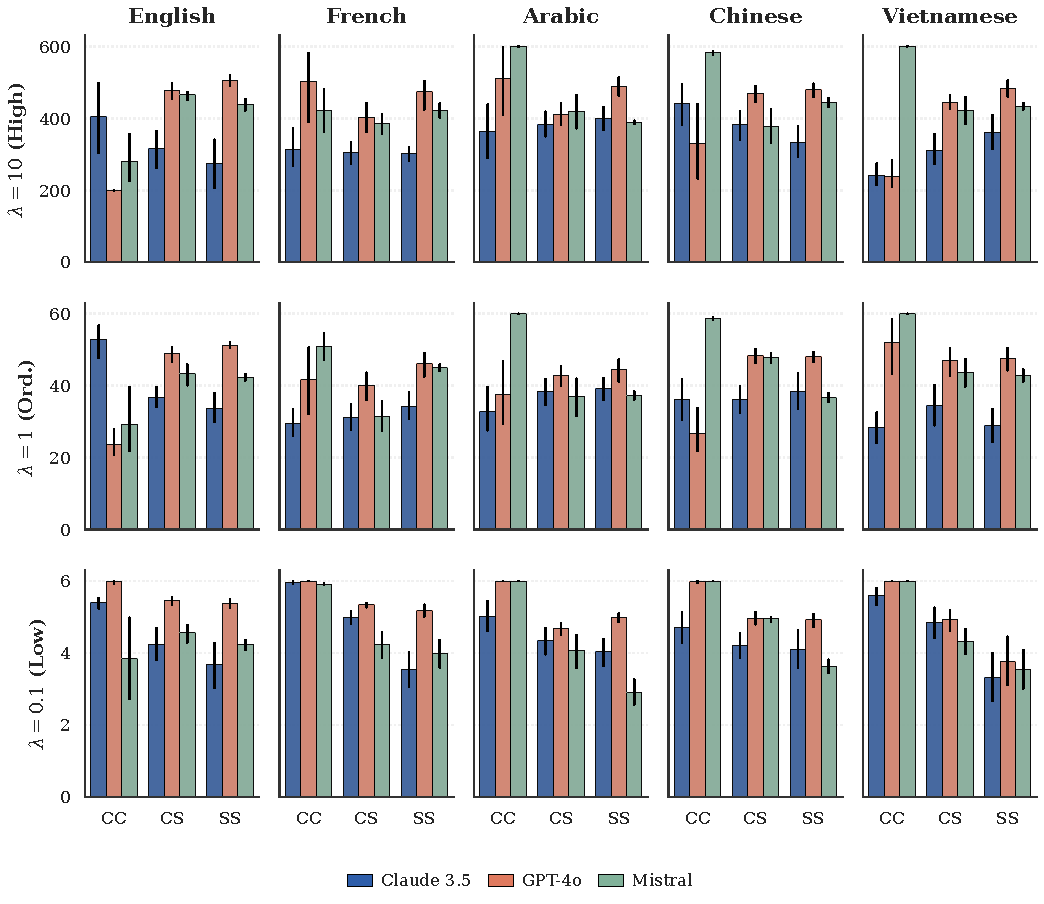
\includegraphics[width=\linewidth]{all_figures/penalties_subplots.pdf}
    \caption{Aggregated final penalties across repeated Prisoner's Dilemma games for the three proprietary LLMs (Claude~3.5~Haiku, GPT-4o, Mistral~Large) under three payoff scales $\lambda \in \{0.1, 1.0, 10.0\}$. Results are reported across five languages (columns) and three personality pairings (CC, CS, SS, where CS pools the asymmetric CS and SC ``mixed'' pairings). Lower bars indicate better outcomes; error bars are bootstrap intervals over the repetitions within each displayed cell. The $y$-axis is rescaled by an order of magnitude across rows, mirroring the $\lambda$ multiplier, so within-row comparison is the meaningful unit.}
    \label{fig:total_penalties_appendix}
\end{figure}

\subsection{Mixed-strategy labels}\label{appendix:mixture_labels}

The hybrid rule-based component of our classifier emits a \emph{composite} label whenever a trajectory simultaneously satisfies the deterministic rule definitions of more than one canonical strategy (Appendix~\ref{appendix:rule_based}). On the proprietary corpus at the $\tau \geq 0.9$ threshold, $75.6\%$ of high-confidence trajectories receive a single canonical label and $24.4\%$ receive a composite label. Table~\ref{tab:composite_labels} reports the distribution of composite labels.

\begin{table}[!htbp]
\centering
\caption{Composite-label distribution among high-confidence ($\tau \geq 0.9$) proprietary trajectories that simultaneously satisfy more than one canonical rule. ``Share of composite'' is normalised within the composite subset; the composite subset itself accounts for $24.4\%$ of all high-confidence trajectories.}
\label{tab:composite_labels}
\footnotesize
\begin{tabular}{lcc}
\toprule
\textbf{Composite label} & \textbf{Count} & \textbf{Share of composite (\%)} \\
\midrule
ALLD$|$TFT        & 291 & 40.9 \\
ALLC$|$TFT$|$WSLS & 202 & 28.4 \\
ALLD$|$WSLS       & 122 & 17.1 \\
TFT$|$WSLS        &  97 & 13.6 \\
\bottomrule
\end{tabular}
\end{table}

The composite labels cluster around four patterns. The most frequent ALLD$|$TFT pattern corresponds to mutual-defection trajectories where the opponent also defects throughout: the agent's all-defect history simultaneously satisfies ALLD and TFT, because TFT degenerates to ALLD when the opponent never cooperates. The next most frequent ALLC$|$TFT$|$WSLS triple is its mirror image: trajectories of nearly-all-cooperation that simultaneously satisfy ALLC, TFT and WSLS because the latter two strategies coincide with ALLC when no defection ever occurs. Both are structural ambiguities of short trajectories in absorbing mutual-cooperation or mutual-defection regimes rather than signs of genuine mixed play. ALLD$|$WSLS and TFT$|$WSLS reflect the well-known overlap between WSLS and other reactive strategies on short horizons under execution noise~\cite{diStefanoIntention2023,inferenceStrategies,Han2012ALIFEjournal}. Removing the composite trajectories entirely or, alternatively, re-distributing them across their constituent labels under a uniform-mass tie-breaking rule shifts the aggregate frequencies in Table~1 by only a couple of percentage points per strategy and leaves the high-stake reversal documented in Section~3.5 unchanged.

\subsection{Hidden Markov segmentation as a robustness check}\label{appendix:hmm_segmentation}

To complement the rule-based composite-label diagnostic in Appendix~\ref{appendix:mixture_labels}, we fit a four-state Hidden Markov Model on every proprietary trajectory. The four hidden states correspond to the four canonical strategies $\{$ALLC, ALLD, TFT, WSLS$\}$; the emission probability of state $k$ at round $t$ is the memory-one probability that strategy $k$ produces the observed action given the joint history of round $t{-}1$, with a symmetric execution-noise factor $\varepsilon{=}0.05$. The transition matrix is a uniform leak with switching probability $0.1$ at every step. Viterbi decoding then returns the most likely sequence of hidden states.

\begin{table}[!htbp]
\centering
\caption{HMM Viterbi segmentation on the proprietary corpus ($n = 3{,}600$ trajectories): per-$\lambda$ strategy share computed by redistributing each trajectory's mass over the hidden states visited in its Viterbi path. The directional stake effect (ALLD share falling, ALLC share rising as $\lambda$ grows from $0.1$ to $1$) is preserved.}
\label{tab:hmm_per_lambda}
\footnotesize
\begin{tabular}{lccccc}
\toprule
$\lambda$ & $n$ & ALLC (\%) & ALLD (\%) & TFT (\%) & WSLS (\%) \\
\midrule
0.1  & 1{,}200 & 35.16 & 47.98 & 8.33 & 8.53 \\
1.0  & 1{,}200 & 50.12 & 28.34 & 8.40 & 13.13 \\
10.0 & 1{,}200 & 51.38 & 29.82 & 9.09 & 9.71 \\
\bottomrule
\end{tabular}
\end{table}

Two key numbers stand out. First, only $20.2\%$ of trajectories visit more than one hidden state, of the same order as the $24.4\%$ composite-label rate of the rule-based pipeline (Appendix~\ref{appendix:mixture_labels}); the small residual gap is consistent with the HMM's smoothed Viterbi path being slightly less likely to flip between strategies than the strict rule-matching test. The average Viterbi path contains just $0.21$ switches. Second, the redistributed per-$\lambda$ shares in Table~\ref{tab:hmm_per_lambda} reproduce the headline pattern of Section~3.2: ALLD share falls from $48\%$ at $\lambda = 0.1$ to $\approx 30\%$ at $\lambda \in \{1, 10\}$, and ALLC absorbs most of the freed mass. The high-stake cooperation effect is therefore not an artefact of single-label attribution.

\subsection{EGT detailed view across stakes and noise levels}\label{appendix:egt_noise_sweep}

Figures~\ref{fig:egt_full_lambda_by_noise} and~\ref{fig:egt_noise_by_lambda} unpack the two-panel summary in Figure~7 into the full per-strategy view. The first sweeps payoff scale $\lambda$ on a logarithmic grid for three execution-noise levels and reports the stationary frequency of all four canonical strategies; the second holds $\lambda$ fixed at three representative values and sweeps execution noise $\varepsilon$. Both are computed under identical settings ($Z = 100$, $\beta = 0.1$, $r = 10$ rounds, small-mutation limit).

\begin{figure}[!htbp]
    \centering
    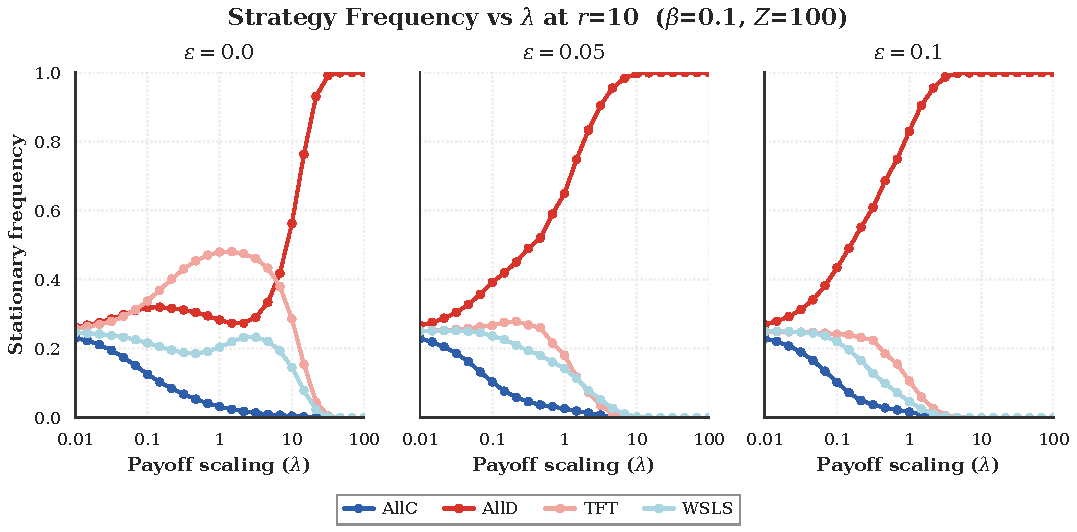
\includegraphics[width=\linewidth]{all_figures/fig10_egt_freq_vs_lambda_by_noise.pdf}
    \caption{\textbf{Stationary strategy frequencies as a function of payoff scaling $\lambda$ for three execution-noise levels $\varepsilon \in \{0,\,0.05,\,0.1\}$ at $r = 10$ rounds.} Each panel reports the long-run frequency of the four canonical strategies (ALLC, ALLD, TFT, WSLS) in a finite well-mixed population ($Z=100$, $\beta=0.1$) under the small-mutation limit, using the FAIRGAME penalty matrix scaled by $\lambda$. ALLD becomes evolutionarily dominant as $\lambda$ grows; introducing implementation noise accelerates the decay of TFT (sharply so at $\lambda = 1$) while the WSLS share decays more gradually, consistent with WSLS's self-correcting advantage.}
    \label{fig:egt_full_lambda_by_noise}
\end{figure}

At very low stakes ($\lambda \lesssim 0.1$) the conditional cooperators TFT and WSLS retain non-trivial mass because the payoff differential between mutual cooperation and mutual defection is too small for ALLD to invade efficiently. As $\lambda$ grows, the relative advantage of ALLD against any partial cooperator widens and the stationary distribution sharply concentrates on ALLD, recovering the classical risk-dominant outcome predicted in finite populations. Modest implementation noise accelerates this collapse, and the effect is sharpest on TFT: at $\lambda = 1$ the TFT share falls from $\approx 48\%$ at $\varepsilon = 0$ to $\approx 15\%$ at $\varepsilon = 0.05$ and $\approx 9\%$ at $\varepsilon = 0.1$, whereas the WSLS share decays more gradually over the same noise range, consistent with WSLS's self-correcting property of switching back to cooperation after mutual defection.

\begin{figure}[!htbp]
    \centering
    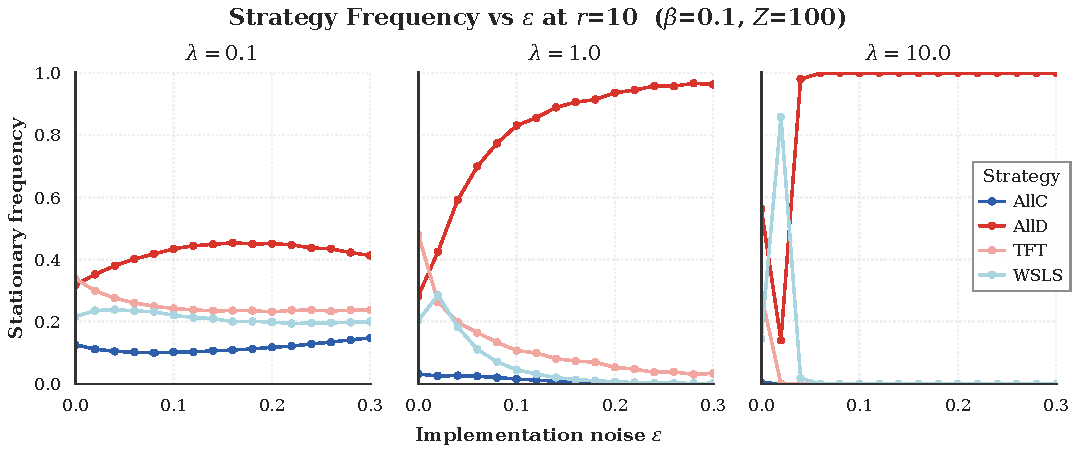
\includegraphics[width=\linewidth]{all_figures/fig11_egt_freq_vs_noise_by_lambda.pdf}
    \caption{\textbf{Stationary strategy frequencies as a function of execution noise $\varepsilon$ for three payoff scales $\lambda \in \{0.1,\,1,\,10\}$ at $r = 10$ rounds.} Population, selection intensity, and SML treatment are identical to those of Figure~\ref{fig:egt_full_lambda_by_noise}. At low stakes ($\lambda = 0.1$), execution noise erodes the conditional cooperators asymmetrically: TFT remains the modal conditional strategy across the whole noise range, but its share decays by $\approx 11$ percentage points as $\varepsilon$ goes from $0$ to $0.3$, while the WSLS share stays roughly flat ($\approx 22$--$26\%$); the freed mass migrates to ALLD. At higher stakes ($\lambda \in \{1,10\}$), the population is locked into ALLD irrespective of $\varepsilon$.}
    \label{fig:egt_noise_by_lambda}
\end{figure}

Holding $\lambda$ fixed and sweeping $\varepsilon$ makes the noise-tolerance asymmetry directly visible: at $\lambda = 0.1$, where ALLD is least dominant, increasing $\varepsilon$ erodes the conditional cooperators with a steeper drop on TFT than on WSLS, and the freed mass migrates to ALLD; at $\lambda \in \{1, 10\}$ the population is locked into ALLD regardless of $\varepsilon$.

\subsection{Baseline FAIRGAME analysis: detailed results}\label{appendix:baseline_fairgame}

This appendix presents the complete analysis of LLM strategic behaviour from the baseline FAIRGAME dataset, complementing the payoff-scaled experiments in the main text. The dataset covers four LLM models - Claude~3.5~Sonnet, Llama~3.1~405B~Instruct, Mistral~Large, and GPT-4o - across five languages (Arabic, Chinese, English, French, and Vietnamese).

\subsubsection{Hybrid classification approach}

While our LSTM model demonstrates strong performance in strategy classification, it was originally designed as a single-label classifier. To address this limitation and ensure comprehensive coverage, we adopt a hybrid labelling approach that combines model predictions with rule-based strategy assignment (see Appendix~\ref{appendix:rule_based}).

\subsubsection{Strategy distribution across models}

\begin{figure}[!htbp]
    \centering
    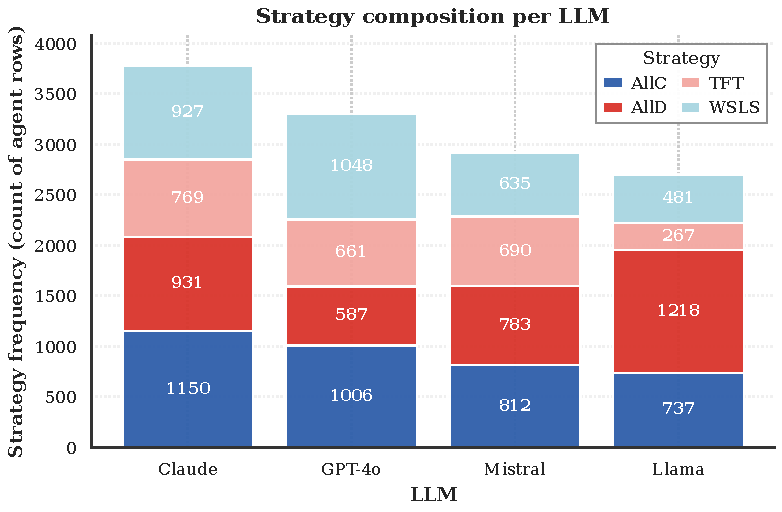
\includegraphics[width=0.9\linewidth]{all_figures/fig_strategy_by_model_stacked.pdf}
    \caption{Strategic behavioural composition of four LLMs in the iterated Prisoner's Dilemma. Each stacked column shows the absolute count of agent--game rows assigned to each strategy by the hybrid LSTM + rule-based classifier on the baseline FAIRGAME corpus (1{,}200 games per model $\times$ 2 agents per game = 2{,}400 base rows; composite labels such as ``ALLD$|$WSLS'' are expanded into one row per component, yielding the totals annotated on each bar).}
    \label{fig:strategy_distribution_appendix}
\end{figure}

The strategic preference analysis from the \emph{baseline FAIRGAME dataset} ($4{,}800$ games pooled across four models, $12{,}702$ rows after composite expansion) reveals heterogeneity in decision-making across LLM architectures. Claude~3.5~Sonnet is mildly cooperative-leaning but otherwise balanced: ALLC ($30.4\%$) is the modal strategy, with ALLD ($24.6\%$), WSLS ($24.5\%$) and TFT ($20.4\%$) all within five percentage points of each other. Llama~3.1~405B~Instruct is the only defection-dominant model: ALLD ($45.1\%$) accounts for nearly half of its rows, while TFT ($9.9\%$) and WSLS ($17.8\%$) are correspondingly suppressed. Mistral~Large produces the flattest distribution of any model in our corpus, with the four strategies occupying $27.8\%$ (ALLC), $26.8\%$ (ALLD), $23.6\%$ (TFT) and $21.7\%$ (WSLS). Finally, GPT-4o is the most reciprocity-tilted: WSLS ($31.7\%$) and ALLC ($30.5\%$) jointly account for $62.2\%$ of its rows, with ALLD held to $17.8\%$.\footnote{GPT-4o exhibits a markedly higher ALLD share in the payoff-scaled experiments of the main paper, where stake magnitude rather than language is the manipulation of interest. The baseline corpus reported here fixes $\lambda$ at the FAIRGAME default and therefore captures a different operating point of the same model.}

\subsubsection{Language effects on strategies}

\begin{figure}[!htbp]
    \centering
    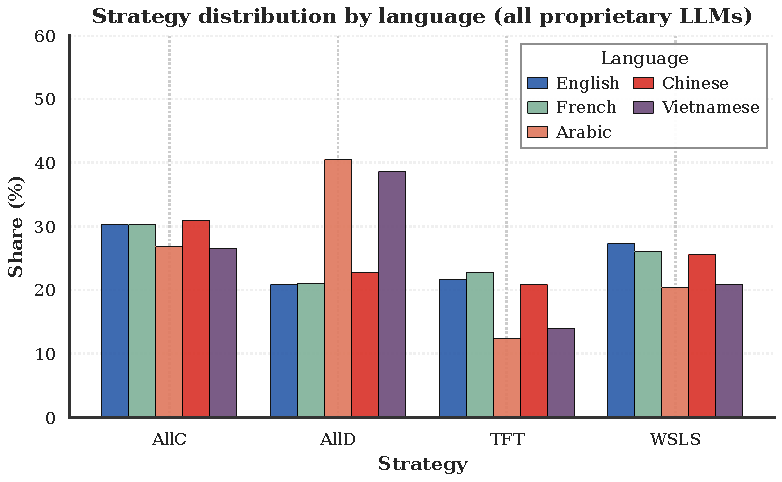
\includegraphics[width=0.75\linewidth]{all_figures/fig_strategy_by_language.pdf}
    \caption{Strategy distribution across languages on the baseline FAIRGAME dataset, pooled across all four proprietary LLMs. Arabic and Vietnamese stand apart with markedly higher ALLD shares, while English, French and Chinese cluster together at much lower defection rates.}
    \label{fig:language_effect_appendix}
\end{figure}

\begin{figure}[!htbp]
    \centering
    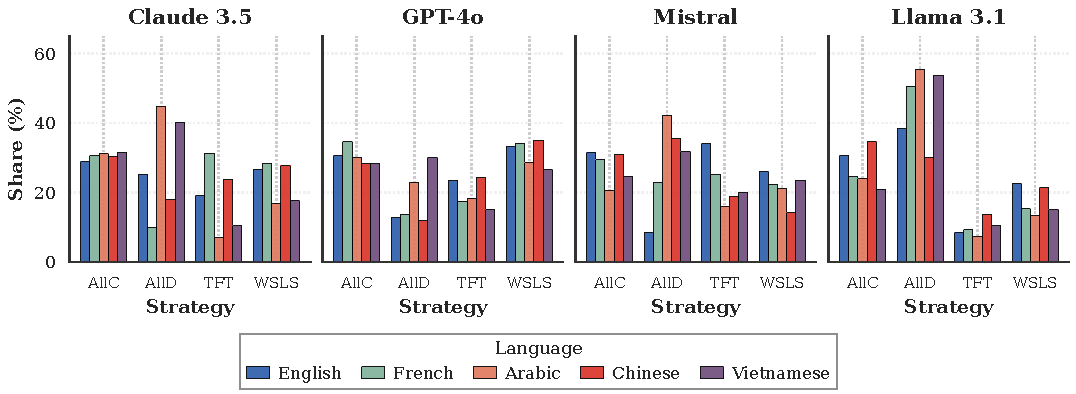
\includegraphics[width=\linewidth]{all_figures/fig_strategy_by_language_per_model.pdf}
    \caption{Strategy distribution by language, faceted per LLM (Claude~3.5, GPT-4o, Mistral, Llama~3.1~405B). The Arabic/Vietnamese vs.\ English/French/Chinese cluster split observed in Figure~\ref{fig:language_effect_appendix} is reproduced inside every model, so it is not driven by any single LLM's idiosyncrasies.}
    \label{fig:language_effect_per_model_appendix}
\end{figure}

The language of the interaction has a substantial and direction-consistent effect on the strategic mix. Pooling all four models, the five languages split into two clusters along the defection axis: Arabic ($40.5\%$ ALLD) and Vietnamese ($38.6\%$ ALLD) sit roughly twenty percentage points above English ($20.8\%$), French ($21.0\%$) and Chinese ($22.8\%$), which are statistically indistinguishable from each other on this metric. The same cluster boundary reappears, with mirror symmetry, in the conditional strategies: English ($27.3\%$ WSLS, $21.6\%$ TFT), French ($26.0\%$, $22.8\%$) and Chinese ($25.5\%$, $20.8\%$) all carry between forty and fifty percent of their probability mass on the two reciprocal strategies, whereas Arabic ($20.4\%$, $12.4\%$) and Vietnamese ($20.9\%$, $14.0\%$) carry only about a third. The unconditional cooperation share is far less language-sensitive, ranging only from $26.6\%$ (Vietnamese) to $30.9\%$ (Chinese). Figure~\ref{fig:language_effect_per_model_appendix} shows that this two-cluster pattern is reproduced inside every model, so it is not driven by any one LLM's idiosyncrasies.

\subsubsection{The language effect: agent scores and strategy mix}\label{appendix:ml}

\noindent\textbf{The language effect (baseline dataset).} \emph{The following analysis is restricted to the baseline FAIRGAME dataset (Claude~3.5~Sonnet, Llama~3.1~405B, GPT-4o, Mistral~Large) and is independent of the payoff-scaled experiments in the main paper; the language patterns reported here are baseline-corpus effects.}

Figure~\ref{fig:language_effect} combines two complementary views of the language effect. Panel~(a) reports the per-agent total score (sum of per-round penalties) averaged across all games in each language. Two regularities stand out. First, Agent~2 outperforms Agent~1 in every language; the average gap is $9.0$ penalty points and is largest in Arabic ($12.0$) and English ($12.0$), suggesting a structural second-mover advantage in the FAIRGAME prompt template. Second, the language-by-language ordering of agent payoffs is itself informative: Arabic ($47.79$ / $59.82$) and Vietnamese ($49.99$ / $55.69$) yield the highest absolute scores -- consistent with the elevated ALLD rates documented in Figure~\ref{fig:language_effect_appendix} above, since defection is the higher-payoff strategy in a one-shot Prisoner's Dilemma -- while English ($41.41$ / $53.37$) and French ($41.90$ / $51.33$) yield the lowest, consistent with their higher conditional-cooperation rates.

Panel~(b) shows the same strategy-by-language crosstab as the top sub-panel of Figure~\ref{fig:language_effect_appendix} and confirms two structural patterns. (i)~The languages cluster into a ``defection-leaning'' bloc (Arabic, Vietnamese: ALLD $\approx 40\%$) and a ``reciprocity-leaning'' bloc (English, French, Chinese: ALLD $\approx 21\%$); the gap on this single axis is approximately twenty percentage points. (ii)~Within the reciprocity-leaning bloc, the three languages are nearly interchangeable -- their WSLS shares lie in a narrow $25.5$--$27.3\%$ band and their TFT shares in $20.8$--$22.8\%$ -- so any individual claim of a uniquely ``Chinese TFT'' or ``French WSLS'' signature would be unsupported by these data. Unconditional cooperation (ALLC), by contrast, is essentially flat across languages ($26.6$--$30.9\%$), so the language effect operates mainly through the conditional/unconditional defection trade-off rather than through cooperative behaviour per se. These findings indicate that the prompt language modulates whether the model retrieves a contingent-reciprocity or a one-shot defection script, rather than uniformly tilting it toward cooperation or competition.

\begin{figure}[!htbp]
    \centering
    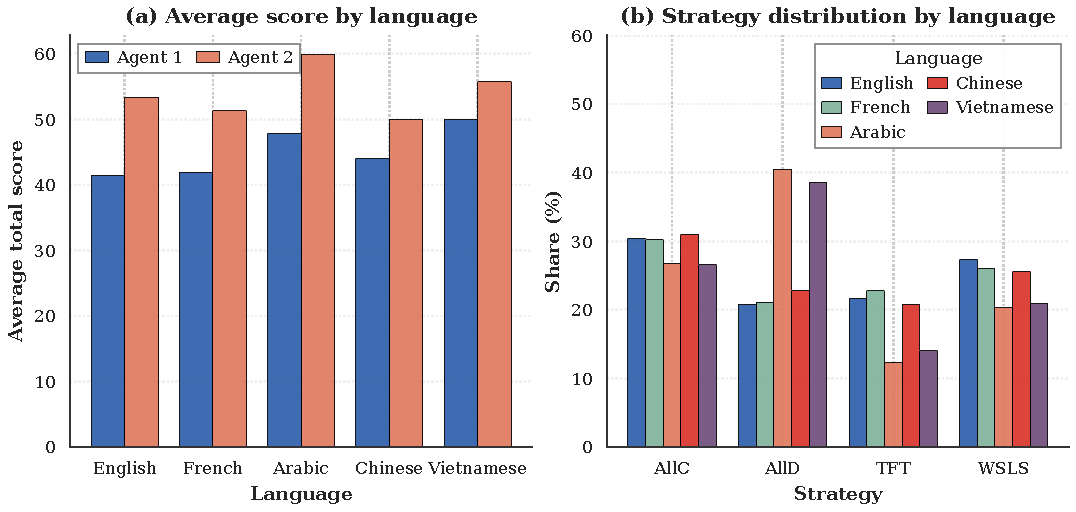
\includegraphics[width=\linewidth]{all_figures/fig_language_effect_2panel.pdf}
    \caption{\textbf{The language effect.} (a) Mean cumulative per-agent score by prompt language (sum of per-round penalties; higher = more total payoff). Agent~2 outperforms Agent~1 in every language, and absolute scores are highest in Arabic and Vietnamese -- the same languages that elicit the highest ALLD rates in panel~(b). (b) Strategy distribution by language pooled across all four LLMs: Arabic and Vietnamese cluster apart from English, French and Chinese on the ALLD axis, while ALLC is approximately language-invariant.}
    \label{fig:language_effect}
\end{figure}

\subsection{Open-weight small LLMs: robustness checks}\label{appendix:small_llm_robustness}

Four follow-up analyses substantiate the open-weight small-LLM results reported in Section~3.6. They are grouped here for clarity: the per-condition penalty breakdown provides the full cell-level view of mean penalties across languages and personality pairings; horizon robustness checks that the directional stake effect is detectable already in the first ten rounds; confidence-threshold robustness checks that the model-level heterogeneity is not driven by the $\tau = 0.9$ cutoff; and the chi-square test quantifies the stake effect on this corpus.

\subsubsection{Per-condition penalty breakdown (open-weight small LLMs)}\label{appendix:small_per_condition_penalties}

The companion of Figure~\ref{fig:total_penalties_appendix} for the open-weight small LLMs: Figure~\ref{fig:small_penalties} reports the per-cell mean penalties across the full six-multiplier sweep of the open-weight corpus ($\lambda \in \{0.01, 0.1, 1, 10, 100, 1000\}$); the middle rows ($\lambda \in \{0.1, 1, 10\}$, marked Low/Ord./High) match the three stake regimes of the proprietary analysis. The picture is qualitatively similar: cooperative pairings (CC) consistently incur lower penalties than selfish ones (SS); per-language differences are model-specific; and the Arabic prompts again elicit elevated defection in cooperative pairings.

\begin{figure}[!htbp]
    \centering
    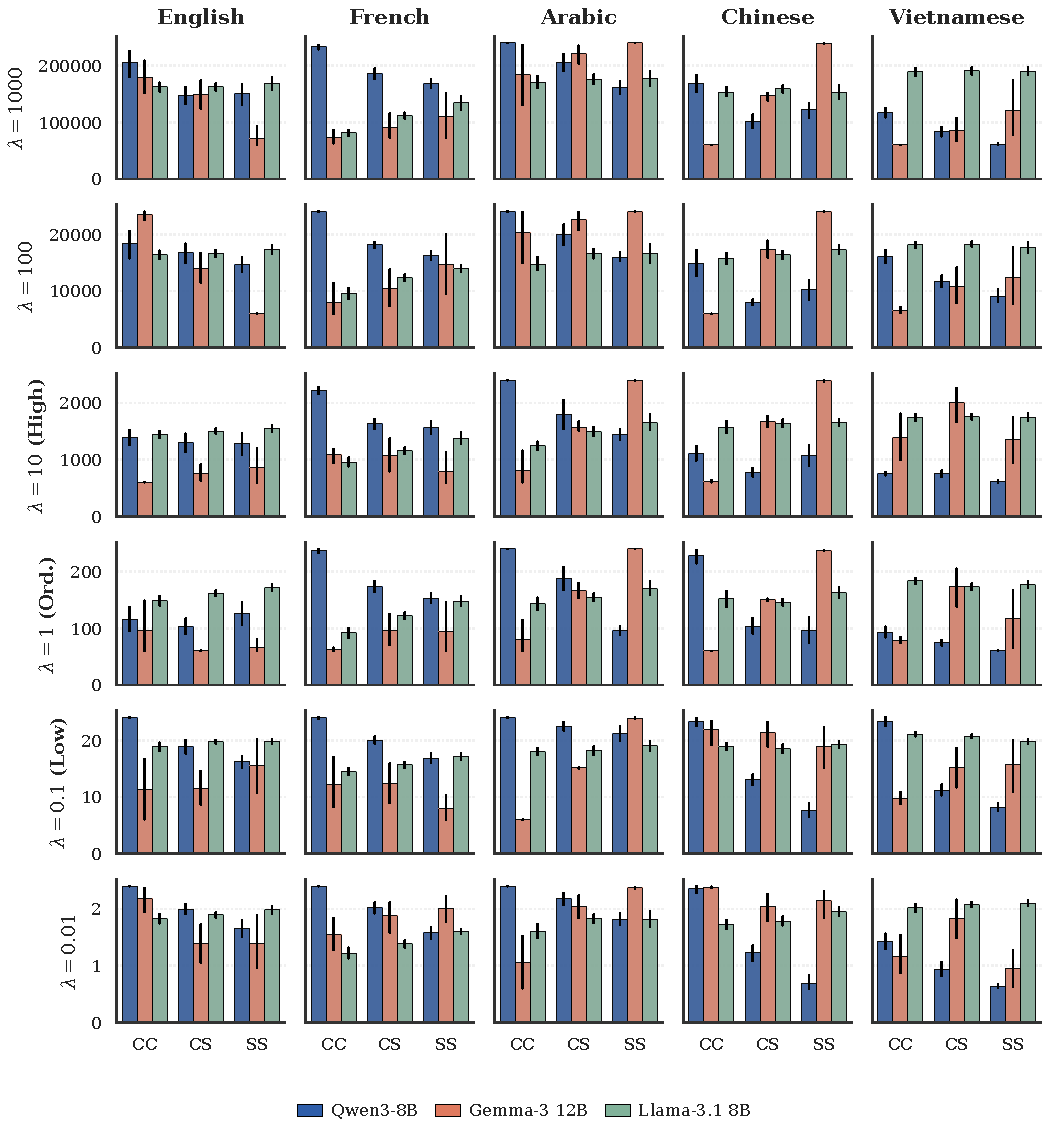
\includegraphics[width=\linewidth]{all_figures/fig_small_penalties_subplots.pdf}
    \caption{Per-condition penalties for the three open-weight LLMs under the payoff-scaled Prisoner's Dilemma. Rows are the six stake multipliers of the open-weight sweep, from $\lambda{=}1000$ (top) down to $\lambda{=}0.01$ (bottom); the $\lambda{=}10$ (\textbf{High}), $\lambda{=}1$ (\textbf{Ord.}) and $\lambda{=}0.1$ (\textbf{Low}) rows match the three stake regimes of the proprietary analysis; columns correspond to the prompt language; within each panel the $x$-axis lists the personality pairing (CC, CS, SS, where CS pools the asymmetric CS and SC ``Mixed'' pairings) and the three bars give the per-agent mean penalty for Qwen3~8B (blue), Gemma-3~12B (orange) and Llama-3.1~8B (green). Lower bars indicate better outcomes; error bars are bootstrap intervals over the repetitions within each displayed cell. The $y$-axis is rescaled by an order of magnitude across rows, mirroring the $\lambda$ multiplier, so within-row comparison is the meaningful unit.}
    \label{fig:small_penalties}
\end{figure}

\subsubsection{Horizon robustness}\label{appendix:horizon_robustness}

The open-weight small-LLM runs reported in Section~3.6 use $N{=}30$ rounds, while the proprietary-model runs in Section~3.1 use $N{=}10$. To verify that the directional stake effect identified in the open-weight corpus is detectable already in the first ten rounds -- and thus that the proprietary-vs-small comparison reported in Section~3.6 is not driven by horizon length -- we apply the same strict rule-based classifier of Appendix~\ref{appendix:rule_based} to two parallel sequences for every open-weight agent: the truncated trajectory (rounds 1--10 only) and the full trajectory (rounds 1--30). Table~\ref{tab:horizon_robustness} reports the resulting per-$\lambda$ distributions, pooled across the three open-weight models and five languages.

\begin{table}[!htbp]
\centering
\caption{Rule-based strategy distribution (\%) for the open-weight small LLMs computed on the first $10$ rounds (``$N{=}10$'') versus the full $30$ rounds (``$N{=}30$'') of every agent trajectory. ``NONE'' denotes trajectories that do not satisfy any canonical rule with tolerance $\epsilon_{\text{noise}}{=}0.1$. The truncated and full classifications agree on $85.7\%$ of trajectories overall, and the directional stake effect (ALLD share falling and ALLC share rising as $\lambda$ grows from $0.1$ to $10$) appears already at $N{=}10$.}
\label{tab:horizon_robustness}
\footnotesize
\begin{tabular}{lccccccc}
\toprule
$\lambda$ & Horizon & ALLC & ALLD & TFT & WSLS & NONE & $n$ \\
\midrule
\multirow{2}{*}{$0.1$}  & $N{=}10$ & 32.15 & 47.81 & 2.16 & 0.79 & 17.09 & \multirow{2}{*}{1527} \\
                        & $N{=}30$ & 33.79 & 37.66 & 1.77 & 0.85 & 25.93 & \\
\midrule
\multirow{2}{*}{$1.0$}  & $N{=}10$ & 53.06 & 25.63 & 1.62 & 0.72 & 18.97 & \multirow{2}{*}{1666} \\
                        & $N{=}30$ & 56.72 & 22.51 & 0.48 & 0.18 & 20.11 & \\
\midrule
\multirow{2}{*}{$10.0$} & $N{=}10$ & 50.80 & 26.79 & 1.09 & 0.90 & 20.41 & \multirow{2}{*}{1553} \\
                        & $N{=}30$ & 53.25 & 21.57 & 2.45 & 0.19 & 22.54 & \\
\bottomrule
\end{tabular}
\end{table}

Two observations follow. First, the per-trajectory label assigned on the first $10$ rounds agrees with the label assigned on the full $30$ rounds in $85.7\%$ of cases, indicating that the rule-based classifier is largely horizon-stable on these data. Second, the qualitative pattern of the stake effect -- ALLD share dropping by approximately $20$ percentage points between $\lambda{=}0.1$ and $\lambda{=}1$, and remaining at a similar level at $\lambda{=}10$ -- is reproduced almost identically by the truncated and full classifications. The directional comparison with the proprietary-model corpus reported in Section~3.6 and Figure~13 is therefore not an artefact of horizon length. The slightly higher share of ``NONE'' (unclassifiable) trajectories at $N{=}30$ is consistent with longer sequences accumulating execution errors that push them outside the canonical rule envelopes, an effect that the LSTM-based hybrid pipeline used in the main text actively absorbs via its noise tolerance.

\subsubsection{Confidence-threshold robustness}\label{appendix:small_unfit}

For completeness, Figure~\ref{fig:small_unfit_threshold} reports the unfit-trajectory rate -- the fraction of trajectories left unclassified by the hybrid rule + LSTM pipeline -- as a function of the LSTM-output confidence threshold $\tau$, computed separately for Qwen3~8B, Gemma-3~12B and Llama-3.1~8B on the open-weight payoff-scaled corpus. At the $\tau = 0.9$ threshold used in the main analysis, the unfit rate is $1.2\%$ for Gemma-3~12B, $10.8\%$ for Qwen3~8B and $33.9\%$ for Llama-3.1~8B; the qualitative ordering of models by conditional-cooperation capacity reported in Section~3.6 is preserved across the entire $\tau \in [0.6, 0.95]$ range, confirming that the threshold choice is not the driver of the model-level heterogeneity.

\begin{figure}[!htbp]
    \centering
    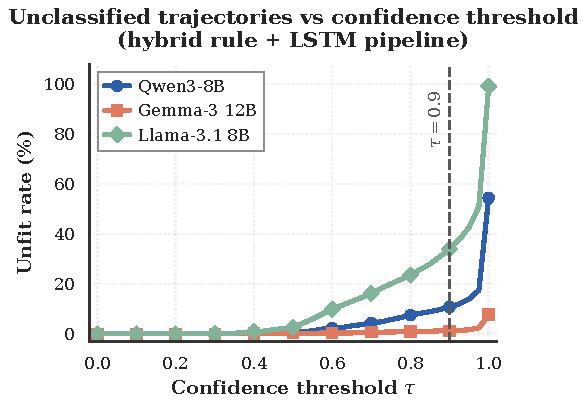
\includegraphics[width=0.8\linewidth]{all_figures/fig_unfit_vs_threshold_small_llm_by_model.pdf}
    \caption{Unfit (non-classifiable) trajectory rate -- the fraction of agent trajectories left unclassified by the hybrid rule + LSTM pipeline -- as a function of the LSTM-output confidence threshold $\tau$ for the three open-weight small LLMs. The dashed vertical line at $\tau{=}0.9$ marks the threshold used in the main analysis, where the unfit rate is $1.2\%$ for Gemma-3~12B, $10.8\%$ for Qwen3~8B and $33.9\%$ for Llama-3.1~8B. Llama-3.1~8B has the largest unfit rate at all $\tau$, consistent with its noisier conditional play.}
    \label{fig:small_unfit_threshold}
\end{figure}

\subsubsection{Chi-square stake-effect test}\label{appendix:small_llm_chi2}

Table~\ref{tab:small_chi2} reports the chi-square test of independence between inferred strategy and stake $\lambda$ for the open-weight small LLMs, both pooled and per model. The test is run on $\tau > 0.9$ high-confidence trajectories at all six multipliers $\lambda \in \{0.01, 0.1, 1, 10, 100, 1000\}$, parallel in spirit to the proprietary-corpus test in Section~3.3. The pooled effect size (Cram\'er's $V \approx 0.10$) is larger than the value observed in the proprietary corpus restricted to three lambdas ($V \approx 0.065$), reflecting the wider stake sweep used here. Per-model, Gemma-3~12B is the least stake-sensitive, consistent with its early-commitment trajectory shape; Llama-3.1~8B is the most sensitive, reflecting its sharp moves between defection-leaning and Tit-for-Tat-dominated regimes; Qwen3~8B sits in between, with the U-shape stake response we noted in the main text.

\begin{table}[!htbp]
\centering
\caption{Chi-square test of independence between inferred strategy and stake $\lambda$ for the open-weight small LLMs at $\tau \geq 0.9$, computed over the full six-multiplier sweep $\lambda \in \{0.01, 0.1, 1, 10, 100, 1000\}$ on the canonical cache (composite labels expanded into one row per matched strategy, identically to Tables~5 and 6). Effect sizes are reported as Cram\'er's $V$.}
\label{tab:small_chi2}
\footnotesize
\begin{tabular}{lccccc}
\toprule
\textbf{Scope} & $n$ & $\chi^2$ & dof & $p$-value & Cram\'er's $V$ \\
\midrule
Gemma-3~12B  & 4{,}663 & 131.16 & 15 & $1.3 \times 10^{-20}$ & 0.097 \\
Qwen3~8B     & 2{,}973 & 143.35 & 15 & $5.0 \times 10^{-23}$ & 0.127 \\
Llama-3.1~8B & 1{,}621 & 227.65 & 15 & $4.9 \times 10^{-40}$ & 0.216 \\
\midrule
Pooled       & 9{,}257 & 274.90 & 15 & $9.0 \times 10^{-50}$ & 0.099 \\
\bottomrule
\end{tabular}
\end{table}


% Flush any still-floating table/figure (e.g. Table B.4) so it is placed with
% its text and never drifts into the reference list below.
\FloatBarrier

% --- Appendix-local reference list (only works cited in this appendix). ---
\printbibliography

\end{document}
